%!TEX root=../root.tex

%%%%%%%%%%%%%%%%%%%%%%%%%%%%%%%%%%%%%%%%%%%%%%%%%%%%%%%%%%%%%%%%%%%%%%%%%%%%%%%%
%2345678901234567890123456789012345678901234567890123456789012345678901234567890
%        1         2         3         4         5         6         7        
\section{MODULAR MODELING}
The main components determining the shape and the dynamics of an \acp{auv} are the hull enclosing electronic internals and the actuators. The actuators can be further divided into thrusters and control fins. For the sake of simplicity and the computability of the overall model in the optimization process, we make the following assumptions:  (i) the hydrodynamic effects on the overall system are dominated by the effects on the hull and fins, those of the thrusters are negligible; (ii) the moment of inertia of the system is assumed to be merely determined by the hull components, fins and thrusters are neglected. 

\subsection{Modeling of Hull Components}
A world inertial frame $\left\{ i \right\}=(x_{i}~y_{i}~z_{i})$ describes the environment of the underwater robot which is fixed in space. The body-fixed reference frame $\left\{ b \right\}=(x_{b}~y_{b}~z_{b})$ for the whole robot is an accelerated coordinate frame fixed to the robot. The origin $o_{b}$ is usually chosen to coincide with the geometric center of the hull which will be referred to as $CO$. The longitudinal axis $x_{b}$ is directed from aft to fore, the transversal axis $y_{b}$ is directed to starboard and the normal axis $z_{b}$ orientates from top to bottom, see Fig.~\ref{FIG:HullThrusterGeometry}.

\begin{figure}[htb]
      \centering
      %\framebox{\parbox{3in}{We suggest that you use a text box to insert a graphic (which is ideally a 300 dpi TIFF or EPS file, with all fonts embedded) because, in an document, this method is somewhat more stable than directly inserting a picture.
%}}
      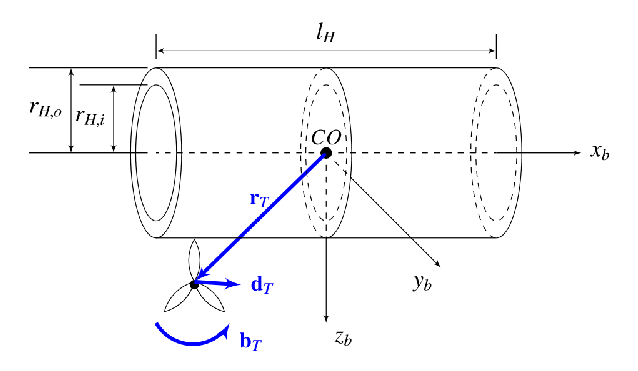
\includegraphics[scale=0.5]{HullThrusterGeometry.eps}
      \caption{Hull and thruster geometry}
      \label{FIG:HullThrusterGeometry}
\end{figure}
The main body typically embeds the navigation- , the sensory-  and the power supply-system. The shell is modeled as a hollow cylinder. We use three parameters to describe the dimensions: the inner radius $r_{H,i}$, the outer radius $r_{H,o}$ and the hull length $l_{H}$. Its mass $m_{H}$ is then calculated as $m_{H}=\rho_{H}\pi(r_{H,o}^{2}-r_{H,i}^{2})l_{H}$, with $\rho_{H}$ being the density of the hull material, and the moment of inertia with respect to its center of gravity can be calculated as follows:
\begin{align*}
I_{H}=diag([I_{xx,H}, I_{yy,H}, I_{zz,H}])
\end{align*}
where $I_{xx,H}=1/2m_{H}(r_{H,0}^{2}+r_{H,i}^{2})$ and $I_{yy,H}=I_{zz,H}=1/4m_{H}(r_{H,o}^{2}+r_{H,i}^{2}+l_{H}^{2}/3)$, due to its rotational symmetry along the $x_b$-axis and the symmetry with respect to the $z_{b}y_{b}-$plane. In the following, we use $r_{H}$ to represent $r_{H,o}$. Within the hull, we model the battery as a solid cylinder with length $l_{H}$ and radius $r_{H}$, the mass $m_{bat}=\rho \pi r_{bat}^{2}l_{bat}$ and the moment of inertia $I_{bat}$ with respect to the battery center of gravity is: 
\begin{align*}
I_{bat}=diag([I_{xx,bat}, I_{yy,bat}, I_{zz,bat}])
\end{align*}
where $I_{xx,bat}=I_{yy,bat}=1/12m_{bat}(3r_{bat}^{2}+l_{bat}^{2})$ and $I_{zz,bat}=1/2m_{bat}r_{bat}^{2}$.
%\begin{figure}[thpb]
     % \centering
      %\framebox{\parbox{3in}{We suggest that you use a text box to insert a graphic (which is ideally a 300 dpi TIFF or EPS file, with all fonts embedded) because, in an document, this method is somewhat more stable than directly inserting a picture.
%}}
     % 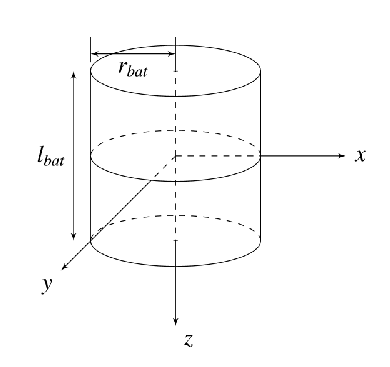
\includegraphics[scale=0.75]{BatModeling.eps}
     % \caption{Modeling of battery as solid cylinder}
     % \label{BatModel}
%\end{figure}
For all other electronic devices, we assume they have a constant mass $m_{d}$, volume $V_{d}$ and moment of inertia $I_{d}$ with respect to the robot body axes $\lbrace b \rbrace$.
For different underwater robot prototypes, the main customizable decision variables for the hull are its length $l_{H}$ and radius $r_{H}$ to enclose all internal devices and influence buoyancy. Therefore, we choose them as the decision variables of hull geometry and obtain the following definition:
\begin{definition}
The geometric decision parameters for the hull $\mathfrak{d}_{H}$ are defined as $\mathfrak{d}_{H}=\lbrace~l_{H}, r_{H}~|~l_{H}\in \mathbb{R}^{+}, r_{H} \in \mathbb{R}^{+}~\rbrace$, where $l_{H}$ denotes the length of the hull cylinder and $r_{H}$ is the radius of the hull cylinder.
\end{definition}
\subsection{Modeling of Thrusters}
As shown in Fig.~\ref{FIG:HullThrusterGeometry}, each thruster is parameterized by the motor orientation $\vec{d}_{T}$ (unit vector), the motor position $\vec{r}_{T}$ in the body frame $\lbrace b \rbrace$ and the motor spin direction $b_{T}\in \lbrace -1,1 \rbrace$, where -1 means counterclockwise and 1 represents clockwise. We use $u_{T}$ and $m_{T,r}$ to denote the magnitude of the thrust force and torque generated by the propeller rotation, respectively.
%\begin{figure}[thpb]
%      \centering
%      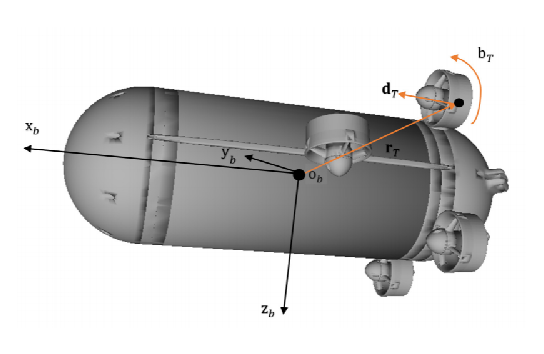
\includegraphics[scale=0.75]{thrusterlocation.eps}
%      \caption{Definition of thruster geometry}
%      \label{FIG:ThrusterLocation}
%\end{figure}
A simple one-state model for the propeller is proposed by~(\cite{c8}). If the propeller rotates in a steady state, the torque $m_{T,r}$ due to the rotation of a propeller is proportional to the thrust force. Thus, we can represent their relationship as $ m_{T,r}=\lambda_{T}u_{T}$, where $\lambda_{T}$ is the torque-force ratio. Taking the thruster motor orientation and the spin direction into consideration, we can obtain the rotation torque vector in $\lbrace b \rbrace$ as $\vec{m}_{T,r}=b_{T}\lambda_{T}u_{T}\vec{d}_{T}$. In addition, the thrust force will produce the thrust torque $\vec{m}_{T,t}$ relative to the center of gravity $CG$ of the complete robot. $CG$ is assumed to be located at the origin $CO$ of the body frame $\lbrace b \rbrace$. Then, the thrust torque can be calculated as $\vec{m}_{T,t}=\vec{r}_{T} \times u_{T}\vec{d}_{T}$, where $\vec{r}_{T} = (x_{T}~y_{T}~z_{T})^{T} \in \mathbb{R}^{3}$ is the position vector of the thruster in the body frame $\lbrace b \rbrace$. Combining the thrust torque and the rotation torque, we express the total torque produced by a thruster as $\vec{m}_{T}=\vec{m}_{T,r}+\vec{m}_{T,t}$. The force direction is determined by the thruster motor orientation $\vec{d}_{T}$ and the force vector $\vec{f}_{T}$ is written as $\vec{f}_{T}=u_{T}\vec{d}_{T} \in \mathbb{R}^{6}$. The generalized force vector $\vec{\tau}_{T}$ generated by a thruster is defined as $\vec{\tau}_{T}=(\vec{f}_{T}~\vec{m}_{T})^{T}\in \mathbb{R}^{6}$. If we treat the thrust force $u_{T}$ as the control input, we can define a unique vector $B_{T}$ mapping the thrust $u_{T}$ to the generalized force $\vec{\tau}_{T}$ as 
\begin{equation}
B_{T}=\begin{bmatrix}
\vec{d}_{T} \\
b_{T}\lambda_{T}\vec{d}_{T}+\vec{r}_{T} \times \vec{d}_{T}
\end{bmatrix} \in \mathbb{R}^{6}.
\end{equation}  
The generalized force produced by thrust force can thus be calculated as $\vec{\tau}=B_{T}u_{T}$. For the thrusters, we choose the geometric decision variables as follows:
\begin{definition}
The geometric parameter set for the thrusters $\mathfrak{d}_{P}$ is defined as $\mathfrak{d}_{P}=\lbrace~b_{T}, \vec{d}_{T}, \vec{r}_{T}~|~b_{T}\in \lbrace -1, 1 \rbrace, \vec{d}_{T} \in \mathbb{R}^{3}, \vec{r}_{T} \in \mathbb{R}^{3}~\rbrace$, where $b_{T}$ denotes the motor spin direction, $\vec{d}_{T}$ is the motor orientation and $\vec{r}_{T}$ represents the motor position.
\end{definition}
\subsection{Modeling of Control Fins}
The fins are approximated as rectangle with length $a_{F}$, width $b_{F}$ and negligible thickness. We assume the side edge $b_{F}$ is directly attached to the hull surface. The fins have a controllable \ac{dof} around an axis parallel to $a_{F}$ in the midsection of $b_{F}$. We represent the position and the orientation of the fins in the hull cylindrical coordinate system as illustrated in Fig.~\ref{FIG:FinGeo}, where $x_{F}$ is defined as the $x_b$-coordinate of the fin geometric center in robot body frame $\lbrace b \rbrace$. Then we rotate the $x_{b}z_{b}$-plane in the counterclockwise direction around $x_b$ by angle $\gamma_{F}$ until the fin geometric center is located in this plane. 
\begin{figure}[thpb]
\centering
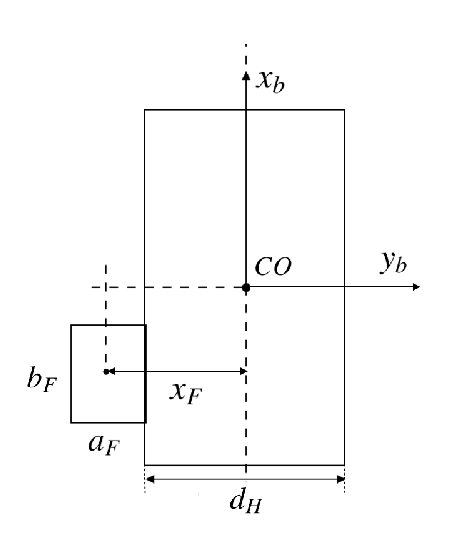
\includegraphics[width=1.25in]{finlocation1.eps}
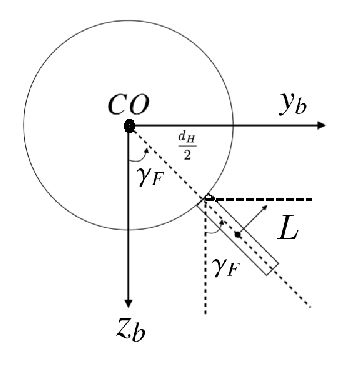
\includegraphics[width=1.25in]{finlocation2.eps}
\caption{Definition of fin geometry}
\label{FIG:FinGeo}
\end{figure}
As a result, the fin geometric center $\vec{r}_{F}$ in the robot body frame $\lbrace b \rbrace$ can be written as
\begin{equation}
\vec{r}_{F}=
\begin{bmatrix}
x_{F}\\0.5(d_{H}+a_{F})\sin(\gamma_{F})\\0.5(d_{H}+a_{F})\cos(\gamma_{F})
\end{bmatrix} \in \mathbb{R}^{3}.
\end{equation}
The unit vectors $\vec{e}_{1}=(0~0~1)^{T}$, $\vec{e}_{2}=(0~1~0)^{T}$ and $\vec{e}_{3}=(1~0~0)^{T}$ are the standard orthonormal basis of the robot body frame. 
We assume the fin velocity $\vec{v}_{fin}$ is equal to the robot velocity $\vec{v}$. For each fin, the lift $\vec{L}$ and drag $\vec{D}$ of fins can be calculated as
\begin{equation}
\vec{L}=0.5 \rho a_{F}b_{F}C_{L}(\alpha)||\vec{v}||^{2}
\begin{bmatrix}
0\\ \cos(\gamma_{F}) \\ -\sin(\gamma_{F})
\end{bmatrix} \in \mathbb{R}^{3},
\end{equation} and 
\begin{equation}
\vec{D} = 0.5 \rho a_{F}b_{F}C_{L}(\alpha)||\vec{v}||^{2}\vec{e}_{1} \in \mathbb{R}^{3},
\end{equation}
where $a_{F}$ and $b_{F}$ are the length and the width of the fin, respectively. $C_{L}$ is the lift coefficient and $C_{D}$ represents the drag coefficient, both of which are dependent on the angle of attack $\alpha$. Assuming the robot mainly moves forward, the surge velocity $u$ is dominant with respect to the sway $v$ and heave velocity $w$. Consequently, we can approximate $||\vec{v}||$ with $u$. Suppose the robot has $n_{f}$ fins, then the resultant force vector produced by all fins can be calculated as
\begin{equation}
\vec{f}_{F}(\alpha_{i})=
\begin{bmatrix}
\sum _{ i=1 }^{ n_{f} }{ \vec{L}_{ i }(\alpha _{ i })^{ T }\vec{e}_{ 1 }+ } \sum _{ i=1 }^{ n_{f} }{ \vec{D}_{ i }(\alpha _{ i })^{ T }\vec{e}_{ 1 } }  \\ \sum _{ i=1 }^{ n_{f} }{\vec{L}_{ i }(\alpha _{ i })^{ T }\vec{e}_{ 2 }+ } \sum _{ i=1 }^{ n_{f} }{ \vec{D}_{ i }(\alpha _{ i })^{ T }\vec{e}_{ 2 } }  \\ \sum _{ i=1 }^{ n_{f} }{ \vec{L}_{ i }(\alpha _{ i })^{ T }\vec{e}_{ 3 }+ } \sum _{ i=1 }^{n_{f} }{ \vec{D}_{ i }(\alpha _{ i })^{ T }\vec{e}_{ 3 } } 
\end{bmatrix} \in \mathbb{R}^{3}.
\end{equation} 
The resultant torque vector is calculated as 
\begin{equation}
\vec{\tau} _{F}(\alpha_{i} )=\sum _{ i=1 }^{n_{f}}{ \vec{r}_{F,i} \times \vec{L}_{i}(\alpha_{i}) } +\sum _{ i=1 }^{n_{f}}{ \vec{r}_{F,i} \times \vec{D}_{i}(\alpha_{i})}
\end{equation}
We regard the lift force as the input force and the drag as a disturbance. For small angles of attack $\alpha$ (about $15^\circ-20^\circ$), it is reasonable to approximate the lift and drag coefficient as $C_{L}(\alpha)=c_{L}\alpha$ and $C_{D}(\alpha)=c_{D}\alpha^{2}$, where $c_{L}$ and $c_{D}$ are fin-specific parameters measured from experiments, respectively. Furthermore, the angle of attack $\alpha$ can be approximated by the mechanical angle of rotation $\delta_{F}$ in the \ac{dof} of the fins. We treat $\delta_{F}$ as the control input for the fin actuators and define a mapping vector for each fin:  
\begin{equation}
B_{F}=\begin{bmatrix}
0\\0.5\rho c_{L}a_{F}b_{F} u^{2}\cos(\gamma_{F})\\
0.5\rho c_{L}a_{F}b_{F} u^{2}\sin(\gamma_{F})\\
-0.25\rho c_{L}a_{F}b_{F} u^{2}\sin(d_{H}+a_{F}) \\
0.5\rho c_{L}a_{F}b_{F} u^{2}x_{F}\sin(\gamma_{F})\\
0.5\rho c_{L}a_{F}b_{F} u^{2}x_{F}\cos(\gamma_{F})
\end{bmatrix} \in \mathbb{R}^{6}
\end{equation}
The fin mapping vector $B_{F}$ depends not only on the geometric parameters but also on the state of the rigid body due the existence of the surge velocity term, while the thruster mapping vector is only geometry-determined. The generalized force generated by the fins can be written as: $\vec{\tau}_{F}=(\vec{f}_{F}~\vec{m}_{F})^{T}=B_{F}\delta_{F}\in \mathbb{R}^{6}$. We select $x_{F}$ and $\gamma_{F}$ as decision variables for the fins:
\begin{definition}
The geometric parameter set for the fins $\mathfrak{d}_{F}$ is defined as $\mathfrak{d}_{F}=\lbrace~x_{F}, \gamma_{F}~|~x_{F}\in \mathbb{R}, \gamma_{F} \in (-\pi,\pi]~\rbrace$, where $x_{F}$ denotes the $x_b$-coordinate of the fin geometric center in the body frame $\lbrace b \rbrace$, $\gamma_{F}$ is the fin placement angle. 
\end{definition}
\subsection{Estimation of the Hydrodynamic Effects}
Hydrodynamic effects (added mass and hydrodynamic damping) are the distinct feature for underwater vehicles. Strictly speaking, each component (hull, thrusters and fins) contributes to the hydrodynamic forces and moments. They depend not only on the robot geometry but also on the inflow fluid velocity. Normally, the underwater robot dynamics are defined in the robot body frame $\lbrace b \rbrace$. However, the hydrodynamic effect of each module is calculated with respect to its own body frame. The calculated hydrodynamic effects need be transformed into the robot body frame $\lbrace b \rbrace$ according to the location of each module in $\lbrace b \rbrace$ to build the robot dynamics. This transformation results in nonlinearities and couplings between robot states and the actuator geometric variables. We assume that the added masses of thrusters and fins are negligible and only the added mass of the cylindrical hull is taken into consideration. The cylindrical hull has three planes of symmetry. The structure of the added mass inertia matrix $M_{A}$ and the added mass Coriolis matrix $C_{A}$ for a vehicle completely submerged in the water can be found in~\cite{c9}. The added mass coefficients can be calculated from the hull geometric parameters: $X_{\dot{u}}=-0.1m_{H}$, $Y_{\dot{v}}=Z_{\dot{w}}=-\pi \rho r_{H}^{2}l_{H}$, $K_{\dot{p}}=0$, $M_{\dot{q}}=N_{\dot{r}}=-1/12\pi \rho r_{H}^{2}l_{H}^{3}$. The damping matrix $D=diag([-X_{u|u|}|u|,-Y_{v|v|}|v|,-Z_{w|w|}|w|,-K_{p|p|}|p|,-M_{q|q|}|q|,-N_{r|r|}|r|])$,\\ the damping coefficients can be also calculated by the hull geometric parameters (see \cite{c10}). The damping coefficient in the $x_b$-direction due to the viscous force acting on the frontal area is given by $X_{u|u|}=-1/2\rho \pi C_{D}r_{H}^{2}$. The damping coefficients in the $y_b$- and $z_b$-axes due to the viscous effects on the side projected area of the hull are given as $Y_{|v|v}=Z_{|w|w}=-1/2\rho C_{D}2r_{H}l_{H}$. The hull has no contribution to the roll moment, hence $K_{p|p|}=0$. The pitch and yaw damping coefficients are equal due to the hull symmetry and given as $M_{q|q|}=N_{r|r|}=-1/12\rho C_{D}r_{H}l_{H}^{4}$ (see \cite{c11}). In this way, we establish the relationship between the explicit values of hydrodynamic terms and the geometric decision variables. 

\subsection{Dynamic Model}
%The moment of inertia of each individual module making up the robot is calculated with respect to the module's own body frame, while the hull frame is usually chosen as the reference body frame for the whole robot. This requires the individual moment of inertia to be transformed to the body frame $\lbrace b \rbrace$. 
%For each submodule whose center of gravity $CG_{s}$ is located in $\vec{r}_{G,s}=(x_{G,s}~y_{G,s}~z_{G,s})^{T}$  and the inertia matrix equals $diag([I_{xx,s}, I_{yy,s}, I_{zz,s}])$ in its own body frame, we can compute their moment of inertia in $\lbrace b \rbrace$ as follows: $I_{xx,s}^{b}=I_{xx,s}+m_{s}(y_{s}^{2}+z_{s}^{2})$, $I_{yy,s}^{b}=I_{yy,s}+m_{s}(z_{s}^{2}+x_{s}^{2})$, $I_{zz,s}^{b}=I_{zz,s}+m_{s}(x_{s}^{2}+y_{s}^{2})$, where $I_{xx,s}^{b}$, $I_{yy,s}^{b}$ and $I_{zz,s}^{b}$ are moments of inertia with respect to the body axes $\lbrace b \rbrace$ of the component $s$.
%Suppose we have totally $N$ components, then the resultant center of mass $\vec{r}_{G}$ for the whole robot is 
%\begin{equation}
%\vec{r}_{G}=\frac{\sum_{s=1}^{N}m_{s}\vec{r}_{G,s}}{\sum_{s=1}^{N}m_{s}}.
%\end{equation}
%$\vec{r}_{G}$ is determined by $\mathfrak{d}_{P}$, $\mathfrak{d}_{H}$ and $\mathfrak{d}_{F}$. 
The state variables of underwater robots can be divided into two groups, i.e., kinematic and dynamic states. Dynamic states consist of three linear and three angular velocities represented in the robot body frame $\lbrace b \rbrace$: $\vec{x}_{dyn}=(\vec{v}~\vec{\omega})^{T}=(u~v~w~p~q~r)^{T} \in \mathbb{R}^{6}$. Kinematic states consist of the position and orientation of the underwater robot in the inertial world frame $\lbrace i \rbrace$: $\vec{x}_{kin}=(\vec{p}~\vec{\eta})^{T}
=(x~y~z~\phi~\theta~\psi)^{T} \in \mathbb{R}^{6}$. The complete states are defined as $\vec{x}=(\vec{x}_{dyn}~\vec{x}_{kin})^{T} \in \mathbb{R}^{12}$. 
The standard underwater robot dynamic equation is given by
\begin{equation}
M\begin{bmatrix}
\dot{\vec{v}} \\
\dot{\vec{w}}
\end{bmatrix}+
C(\vec{v},\vec{w})\begin{bmatrix}
\vec{v} \\
\vec{w}
\end{bmatrix}+
D(\vec{v},\vec{w})\begin{bmatrix}
\vec{v}\\
\vec{w}
\end{bmatrix}+\vec{g}(\vec{\eta})=\vec{\tau}. \label{EQ:RobotDynamics}
\end{equation}
Based on the modular modeling, each term in (\ref{EQ:RobotDynamics}) can be uniquely computed from the predefined groups of geometric decision variables. 
\begin{equation}
M:=M_{RB}(\mathfrak{d}_{H}, \mathfrak{d}_{P}, \mathfrak{d}_{F})+M_{A}(x_{dyn}, \mathfrak{d}_{H})  
\end{equation} 
is the generalized mass matrix of the underwater robot with $M_{RB}$ and $M_{A}$ representing the rigid body mass matrix and the added mass matrix, respectively. Furthermore, 
\begin{equation}
   C(\vec{v},\vec{w}):=C_{RB}(\vec{x}_{dyn}, \mathfrak{d}_{H}, \mathfrak{d}_{P}, \mathfrak{d}_{F})+C_{A}(\vec{x}_{dyn}, \mathfrak{d}_{H})
 \end{equation} is the Coriolis-centripetal matrix (including added mass effects), $D(\vec{x}_{dyn}, \mathfrak{d}_{H})$ is the damping matrix and $\vec{g}(\vec{\eta})$ is the vector of gravitational/buoyancy forces and moments, which can be written in the geometry-dependent form as $\vec{g}({\vec{x}_{kin}, \mathfrak{d}_{H}, \mathfrak{d}_{P}, \mathfrak{d}_{F}})$. $\vec{\tau}$ is the generalized force vector generated by thrusters and control surfaces (fins). We use $\vec{u}_{T}$ and $\vec{u}_{F}$ to denote the control inputs generated by thrusters and fins, respectively. Suppose the robot has $n_{t}$ thrusters and $n_{f}$ fins, then the thruster input vector can be written as $\vec{u}_{T}=(u_{T,1}, \cdots, u_{T,n_{t}})^{T} \in \mathbb{R}^{n_{t} \times 1}$ and the fin input vector is defined as $\vec{u}_{F}=(\delta_{F,1}, \cdots, \delta_{F,n_{f}})^{T} \in \mathbb{R}^{n_{f} \times 1}$. The complete input vector for the robot system is defined as $\vec{u}=(\vec{u}_{T}~\vec{u}_{F})^{T} \in \mathbb{R}^{(n_{t}+n_{f}) \times 1}$. For each actuator, there is a corresponding input mapping vector and we can formulate the thruster input matrix as $B_{a,T}=(B_{T,1} \cdots B_{T,n_{t}})\in \mathbb{R}^{6\times n_{t}}$. The fin input matrix is defined as $B_{a,F}=(B_{F,1} \cdots B_{F,n_{t}})\in \mathbb{R}^{6\times n_{f}}$. Stacking them together, we get the input mapping matrix $B_{a}=(B_{a,T}~B_{a,F})^{T} \in \mathbb{R}^{6 \times (n_{t}+n_{f})}$. Thus, we obtain the relationship $\vec{\tau}=B_{a}\vec{u}$. Given a robot prototype with known geometric data of all components, we can directly construct the dynamic equation for analysis. 

